\documentclass[a4paper,12pt]{article}
\usepackage[spanish]{babel} % Paquete para utilizar el español
\usepackage{palatino} % Para cambiar el tipo de letra

% Reconocimiento de caracteres del idioma Español en LaTeX.
\usepackage[utf8x]{inputenc} % Codificacion de entrada
\usepackage[T1]{fontenc} % Codificacion de fuente
\usepackage{graphicx}

% Cabecera de la "portada"
\title{\textbf{StickMotion:} Editor de posturas, posiciones y movimientos}
\author{\small\textit{Carmona Varo, Fernando; García García, José Manuel; López Fernandez, David;}\\
	\small\textit{Navas Torres, Francisco Javier; Porras Bueno, Javier}}

\begin{document}

  \maketitle % Crea el título y los autores

  \begin{abstract}
    El presente documento se corresponde con el entregable nº 3. El cliente recibirá la descripción informal de la gramática y el nuevo prototipo de la
    interfaz, más accesible, usable e intuitiva, promoviendo así un uso autosuficiente y mejorando la experiencia del usuario con la misma.\\
  \end{abstract}

  \section{Gramática del lenguaje}
  A continuación se describe la gramática de Sticky que se ha desarrollado:
  \begin{itemize}
    \item Todas las instrucciones del lenguaje llevarán el carácter fín de instrucción (';').
    \item Los operadores aritméticos reconocidos son: +, -, *, /, ++, --, \%, \textasciicircum, raiz(x).
    \item El lenguaje es sensible a las mayúsculas y minúsculas.
    \item Tipado dinámico de datos:
          \begin{itemize}
            \item Definición de variables: \textit{\textbf{var} nombreVariable}.
            \item Destrucción de variables: \textit{\textbf{sup} nombreVariable}.
          \end{itemize}
    \item Tipos de variables soportadas: booleanas, enteras, reales y cadenas.
    \item Comentarios: monolínea ('\textbf{//}') y multilínea ('\textbf{/*}' y '\textbf{*/}').
    \item Asignaciones: símbolo igual ('\textbf{=}').
    \item Operadores condicionales: '\textbf{<}', '\textbf{>}', '\textbf{<=}', '\textbf{>=}', '\textbf{==}' y '\textbf{!=}'.
    \item Operadores lógicos: '\textbf{Y}', '\textbf{O}', '\textbf{OX}', '\textbf{NO}', '\textbf{!}'.
    \item Los bloques de código irán encerrados entre llaves ('\{' y '\}').
    \item Construcción de bucles:
          \begin{itemize}
            \item Bucle for: \\
                  \hspace{1.5cm}\textit{\textbf{para} (inicio; fin; incremento) \{ sentencias \}} \\
                  \hspace{1.5cm}\textit{\textbf{para} (inicio; fin; incremento) sentencia}
            \item Bucle while: \\
                  \hspace{1.5cm}\textit{\textbf{mientras} (expresión o variable) \{ sentencias \}}\\
                  \hspace{1.5cm}\textit{\textbf{mientras} (expresión o variable) sentencia}
          \end{itemize}
    \item Estructuras condicionales:
          \begin{itemize}
            \item if: \\
                  \hspace{1.5cm}\textit{\textbf{si} (condición) \{ sentencias \}} \\
                  \hspace{1.5cm}\textit{\textbf{si} (condición)}
            \item if-else: \\
                  \hspace{1.5cm}\textit{\textbf{si} (condición) \{ sentencias \} sino \{ sentencias \}}\\
                  \hspace{1.5cm}\textit{\textbf{si} (condición) sentencia sino \{ sentencias \}}\\
                  \hspace{1.5cm}\textit{\textbf{si} (condición) \{ sentencias \} sino sentencia}\\
                  \hspace{1.5cm}\textit{\textbf{si} (condición) sentencia sino sentencia}
            \item switch: \\
                  \hspace{1.5cm}\textit{\textbf{opcion} (expresión o variable) \{ \\
                           \hspace{1.7cm}\textbf{caso} expresión: \{ sentencias \} \textbf{fincaso}; \\
                           \hspace{1.7cm}... \\
                           \hspace{1.7cm}\textbf{defecto}: \{ sentencias \} \textbf{fincaso}; \\
                           \hspace{1.7cm}\}}
          \end{itemize}
    \item Movimientos del Stickman:
          \begin{itemize}
            \item \textit{\textbf{girar CABEZA} x y z}.
            \item \textit{\textbf{girar} [\textbf{BRAZO} | \textbf{PIERNA}] [\textbf{IZQ} | \textbf{DER}] x y z}.
            \item \textit{\textbf{girar STICKMAN} x y z}.
            \item \textit{\textbf{flexionar} [\textbf{BRAZO} | \textbf{PIERNA}] [\textbf{IZQ} | \textbf{DER}] angulo}.
          \end{itemize}
    \item Inclusión de código fuente: \textit{\textbf{incluir}('rutaAlFichero.stk');}
    \item Definición de funciones: \textit{\textbf{def} nombreFunción( [Parámetro/s] ) \{ ... \}}.
  \end{itemize}

  
  \section{Interfaz de la aplicación}
  Con respecto al prototipo que aparece en el entregable número 2 vemos que algunos elementos permanecen y otros han cambiado.\\

  \begin{figure} [h] \begin{center}
    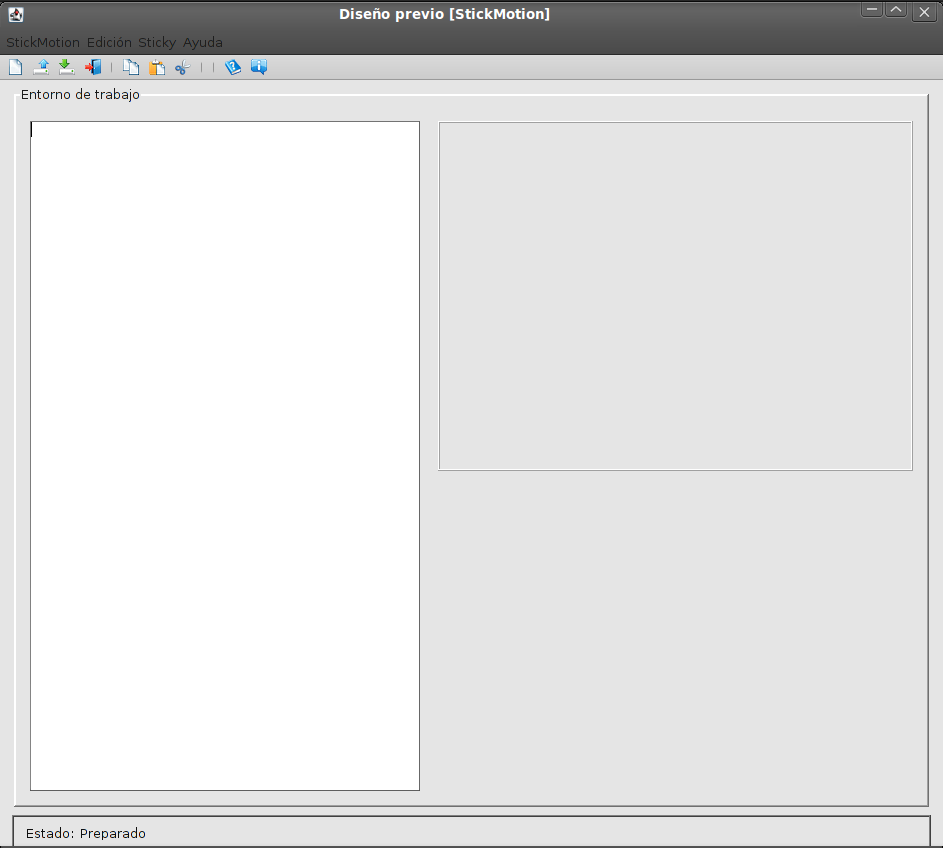
\includegraphics[height=0.95\textwidth]{Interfaz2}
    \caption{Nuevo prototipo de la interfaz de Stickman.} \label{interfaz}
  \end{center} \end{figure}

  A simple vista se observa que el área del editor de texto se ha aumentado para permitir la visualización de una mayor cantidad de código Sticky,
  lo que evitará al usuario el tener que hacer un uso continuado y/o hasta excesivo de las barras de desplazamiento. A su parte derecha se ha 
  desplazado ahora la ventana de animación, quedando aún reservada la parte inferior para los propósitos que aún especifique el cliente, como por
  ejemplo, las acciones maś comunes.\\

  Tal y como se puede apreciar en la figura \ref{detalleBarraHerramientas} se muestra un detalle de una nueva característica: la barra de
  herramientas. Esta nueva función permite que ciertas acciones consideradas como más comunes se puedan llevar a cabo reduciendo el número de clicks
  necesarios por el usuario, facilitando de esta manera su trabajo con la aplicación. Asimismo, cada icono incorpora una breve ayuda sobre el
  objetivo del mismo, muy útil para los usuarios que comienzan a manejar \textit{\textbf{StickMotion}}.
  \begin{figure} [h] \begin{center}
    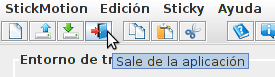
\includegraphics[width=0.6\textwidth]{DetalleTooltip}
    \caption{Áreas de la interfaz de la aplicación.} \label{detalleBarraHerramientas}
  \end{center} \end{figure}
  
  Los iconos que componen dicha barra de herramientas son:
  \begin{itemize}
    \item Ficheros fuente (.stk): nuevo documento, abrir/cargar fichero existente y guardar/salvar el fichero actualmente abierto.
    \item Salir de la aplicación.
    \item Edición de texto: copiar, pegar y cortar.
    \item Ayuda.\\[1cm]
  \end{itemize}

  Las barras de menú y estado permanencen iguales, sin ninguna modificación con respecto al anterior prototipo (entregale nº 2).\\
\end{document}
